\section{Exercise 3.1}
\renewcommand{\labelenumi}{\alph{enumi})}
\begin{enumerate}
\item
Normally, a regular dice has six sides or six options to choose from. In this case, seven dices are cast simultaneously. Therefore, according to the pigeonhole principle, we have seven objects (numbers) placed in six drawers (there are 6 options for each number to be, either 1, 2, 3, 4, 5, or 6). Thus, there must be at least two dice showing the same number. 

\item
By following the example in the text with the column-rule, each column is a drawer and each field is a spot for an object according to the pigeonhole principle. Therefore, a drawer has to contain exactly four objects (as each column must be fully filled, but not more). However, the column-rule states that there can't be more than one of the same number in one column. Since there are four numbers to choose from (and we may have exactly one of each in a column in accordance with the column rule), then there can only be one occurrence of each number in each column. As there are four columns/drawers in a Sudoku-light, it means that the Sudoku-light contains exactly four occurrences of each number 1, 2, 3 and 4. The same line of argument can be used for the row-rule and the sub-square rule.

\item
Since the rules does not have to be obeyed (beyond the fact that we need exactly 4 of each value), it means that the number of ways a Sudoku-light can be filled out, can be calculated as a row of binomial-coefficients:
\[ \begin{pmatrix} 16 \\ 4 \end{pmatrix} \cdot \begin{pmatrix} 12 \\ 4 \end{pmatrix} \cdot \begin{pmatrix} 8 \\ 4 \end{pmatrix} \cdot \begin{pmatrix} 4 \\ 4 \end{pmatrix} = \frac{16!}{4! \cdot 4! \cdot 4! \cdot 4!} = 63.063.000\]

The above is an example of the 4th multinomial (not binomial, or trinomial, but 4), as there are 4 values (choices, which determine the dimension of the multinomial) and there is a restriction on their amount (which determines the values of the numbers in the denominator)

\item
Statement A can be formalized into the following:
\[p \to q \lor r\]

Statement B can be formalized into the following:
\[p \land \neg r \to q\]

The task is to show that the two formulae above are equivalent. In other words:
\[p \to q \lor r \equiv p \land \neg r \to q\]

The above can be solved with the tableau method. If all branches are closed then the two statements are equivalent:

\begin{center}
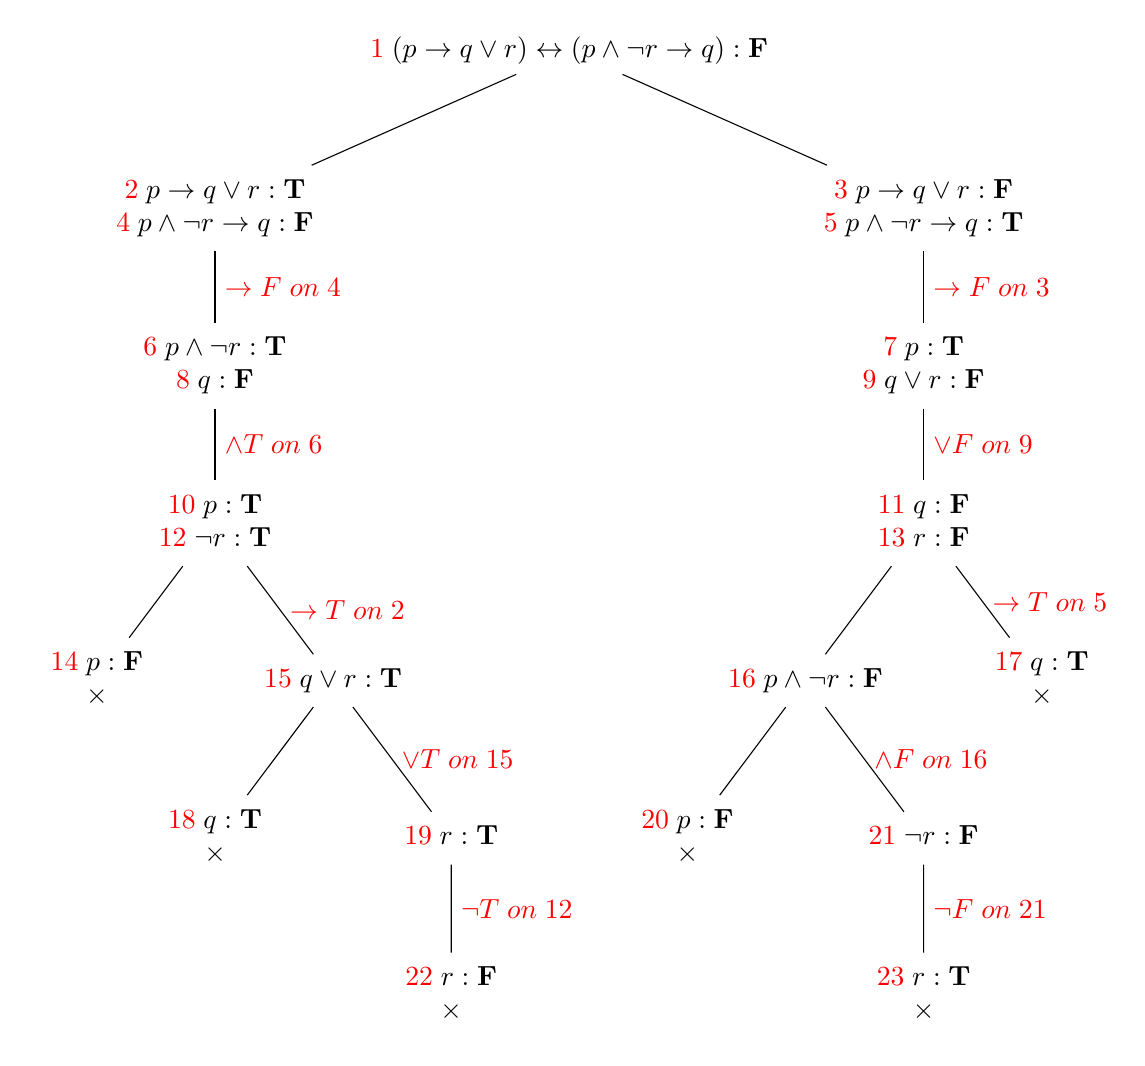
\begin{tikzpicture}
\node {$ \textcolor{red}{1}\; (p \to q \lor r) \leftrightarrow (p \land \neg r \to q):\textbf{F}$} [sibling distance = 9cm] [level distance=20mm] 
        child {node {$ \begin{array}{c} \textcolor{red}{2}\; p \to q \lor r:\textbf{T} \\  \textcolor{red}{4}\; p \land \neg r \to q:\textbf{F} \end{array} $}
                child {node {$ \begin{array}{c} \textcolor{red}{6}\; p \land \neg r:\textbf{T} \\  \textcolor{red}{8}\; q:\textbf{F} \end{array} $}
                    child {node {$ \begin{array}{c} \textcolor{red}{10}\; p:\textbf{T} \\ \textcolor{red}{12}\; \neg r:\textbf{T} \end{array} $} [sibling distance = 3cm]
                            child {node {$ \begin{array}{c} \textcolor{red}{14}\; p:\textbf{F} \\ \times \end{array} $}}
                            child {node {$ \begin{array}{c} \textcolor{red}{15}\; q \lor r:\textbf{T} \end{array} $} [sibling distance = 3cm]
                                child {node {$ \begin{array}{c} \textcolor{red}{18}\; q:\textbf{T} \\ \times \end{array} $}}
                                child {node {$ \begin{array}{c} \textcolor{red}{19}\; r:\textbf{T} \end{array} $}
                                    child {node {$ \begin{array}{c} \textcolor{red}{22}\; r:\textbf{F} \\ \times \end{array} $}
                                        edge from parent node [right, red] {$\neg T\;on\; 12$}} 
                                        edge from parent node [right, red] {$\lor T\;on\; 15$}} 
                                        edge from parent node [right, red] {$\to T\;on\; 2$}}     
                                        edge from parent node [right, red] {$\land T\;on\; 6$}}
                                        edge from parent node [right, red] {$\to F\;on\; 4$}}}
    child {node {$ \begin{array}{c} \textcolor{red}{3}\; p \to q \lor r:\textbf{F} \\  \textcolor{red}{5}\; p \land \neg r \to q:\textbf{T} \end{array} $}
                child {node {$ \begin{array}{c} \textcolor{red}{7}\; p:\textbf{T} \\  \textcolor{red}{9}\; q \lor r:\textbf{F} \end{array} $}
                    child {node {$ \begin{array}{c} \textcolor{red}{11}\; q:\textbf{F} \\ \textcolor{red}{13}\;r:\textbf{F} \end{array} $} [sibling distance = 3cm]
                            child {node {$ \begin{array}{c} \textcolor{red}{16}\; p \land \neg r:\textbf{F} \\ \end{array} $} [sibling distance = 3cm]
                                child {node {$ \begin{array}{c} \textcolor{red}{20}\; p:\textbf{F} \\ \times \end{array} $}}
                                child {node {$ \begin{array}{c} \textcolor{red}{21}\; \neg r:\textbf{F} \\ \end{array} $}
                                    child {node {$ \begin{array}{c} \textcolor{red}{23}\; r:\textbf{T} \\ \times \end{array} $}
                                        edge from parent node [right, red] {$\neg F\;on\; 21$}} 
                                        edge from parent node [right, red] {$\land F\;on\; 16$}} 
                                        edge from parent node [right, red] {}} 
                            child {node {$ \begin{array}{c} \textcolor{red}{17}\; q:\textbf{T} \\ \times \end{array} $}
                                edge from parent node [right, red] {$\to T\;on\; 5$}}     
                                edge from parent node [right, red] {$\lor F\;on\; 9$}}
                                edge from parent node [right, red] {$\to F\;on\; 3$}}};
\end{tikzpicture}
\end{center}

All of the branches in the tableau are closed. Thus, statement A and B are equivalent or in other words $A \equiv B$.

\item
If the column-rule is broken in one column then it's possible to fill out the rest of the Sudoku-light puzzle without breaking the row-rule. However, if the rest of the Sudoku-light is filled out, the column-rule is broken in another column. And you have two columns with the same number appearing twice. Hence, you end in the same situation as described in statement B from the previous exercise d). This situation is visualised down below:

\begin{figure}[h]
\centering
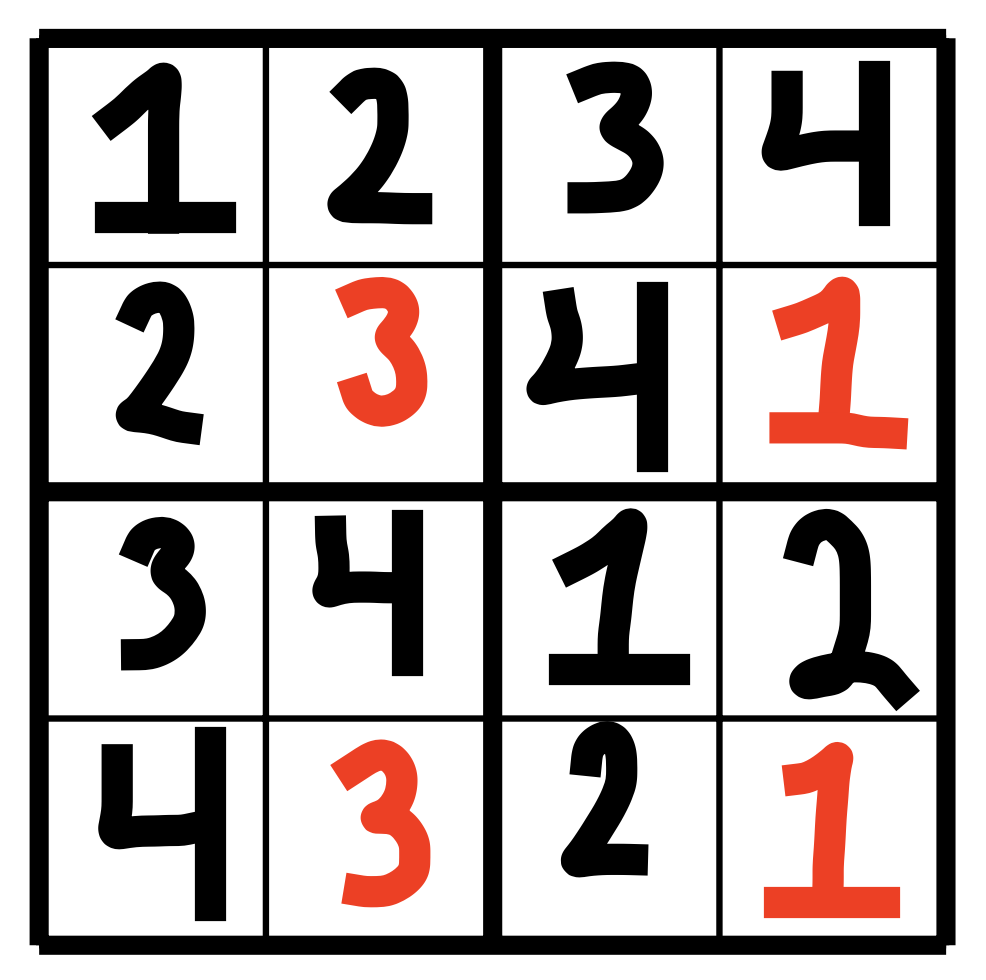
\includegraphics[width=3.2cm]{root/e_1.png}
\end{figure}

In the above picture, the columns breaking the column-rule is highlighted with red.


There's also a situation where both the column-rule and the row-rule are broken simultaneously. If the first column breaks the column-rule then the next two columns can be filled out without breaking the column-rule. This leaves the last column empty. Now, the situation is that one number is already in all four rows but not in the last column. This means that by placing that given number in the last column, then the row-rule will be broken since the number is appearing in all four rows. This situation is visualised down below:

\begin{figure}[h]
\centering
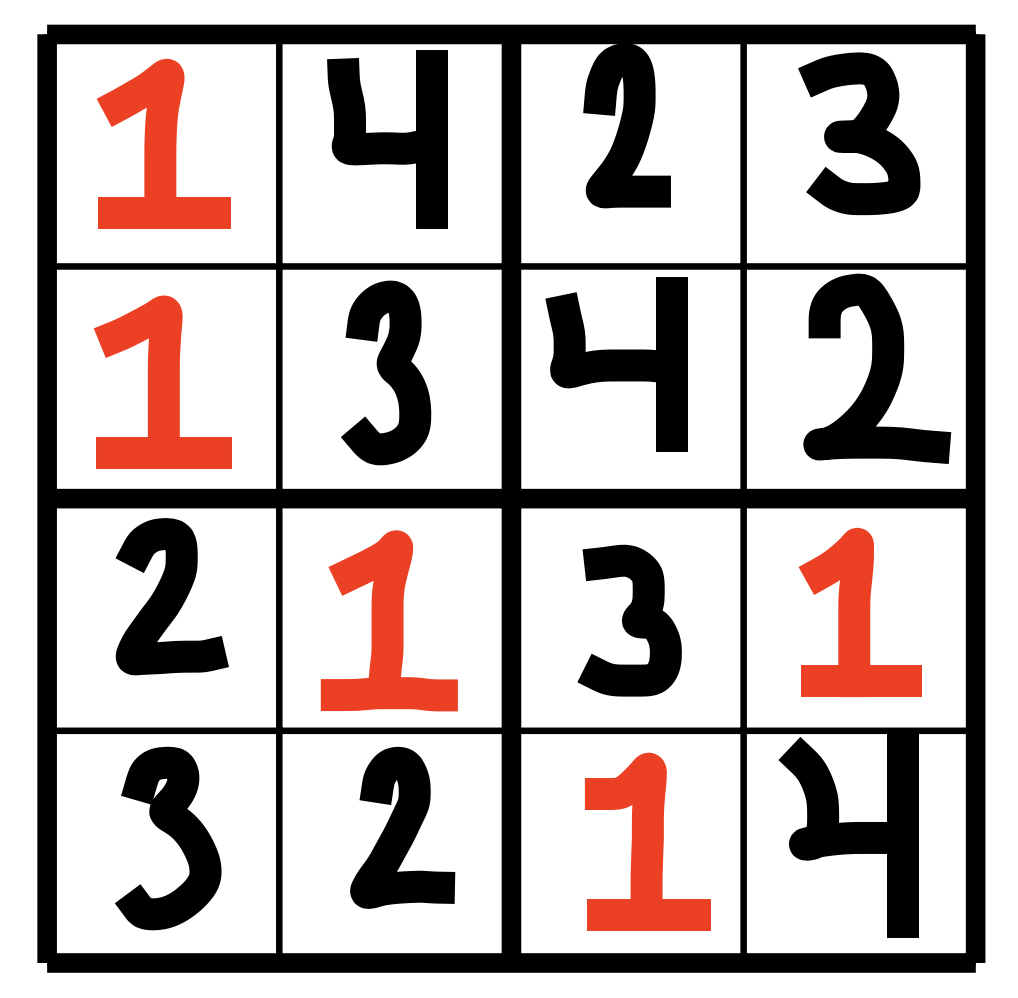
\includegraphics[width=3.2cm]{root/e_2.png}
\end{figure}

\end{enumerate}